% !TEX root = ../main.tex
\chapter{Kiến trúc đề xuất: Hệ thống Đa tác tử ARGOS}\label{chap:argos_proposed}

Chương này trình bày thiết kế và cơ chế vận hành của hệ thống \textbf{ARGOS} (Adaptive Reasoning and Graph Orchestration System). Các điểm nghẽn được xác định tại Chương 3 (thiếu cơ chế tự sửa lỗi, thiếu khả năng nới lỏng ràng buộc, và trọng số truy xuất cố định) được giải quyết bằng cách phân tách các chức năng thành năm tác tử chuyên biệt: Profiler, Graph Agent, Orchestrator, Critic và Relaxation Agent. Các tác tử này liên kết với nhau qua các vòng lặp phản hồi dựa trên mô hình ReAct, tạo nên một kiến trúc có khả năng tự phát hiện lỗi, điều chỉnh chiến lược truy xuất và khôi phục hội thoại khi gặp truy vấn quá khắt khe.

\section{Động lực chuyển đổi sang Vòng lặp phản hồi Đa tác tử (Multi-Agent Feedback Loop)}

Pipeline tuyến tính của GRACE xử lý mỗi truy vấn theo một chiều duy nhất: phân tích ý định → truy xuất → xếp hạng. Khi bước nào thất bại (truy vấn đồ thị trả về rỗng, hay toàn bộ ứng viên bị lọc bởi ràng buộc cứng), pipeline dừng lại và trả về kết quả trống mà không có cơ chế khắc phục. Sự vắng mặt của phản hồi nội bộ (internal feedback) khiến lỗi ở bước đầu lan truyền và khuếch đại qua các bước sau.

ARGOS giải quyết bằng mô hình tổ chức khác: mỗi chức năng cốt lõi được giao cho một tác tử chuyên biệt (Profiler, Graph Agent, Orchestrator, Critic, Relaxation) và các tác tử này giao tiếp qua tín hiệu phản hồi thay vì truyền dữ liệu một chiều. Khi Critic Agent phát hiện không đủ kết quả hợp lệ, nó không trả về lỗi mà phát tín hiệu kích hoạt Relaxation Agent, tác tử này tái cấu trúc ý định và khởi động lại vòng truy xuất. Tổng quan kiến trúc được minh họa trong Hình \ref{fig:argos_architecture}.

\begin{figure}[H]
    \centering
    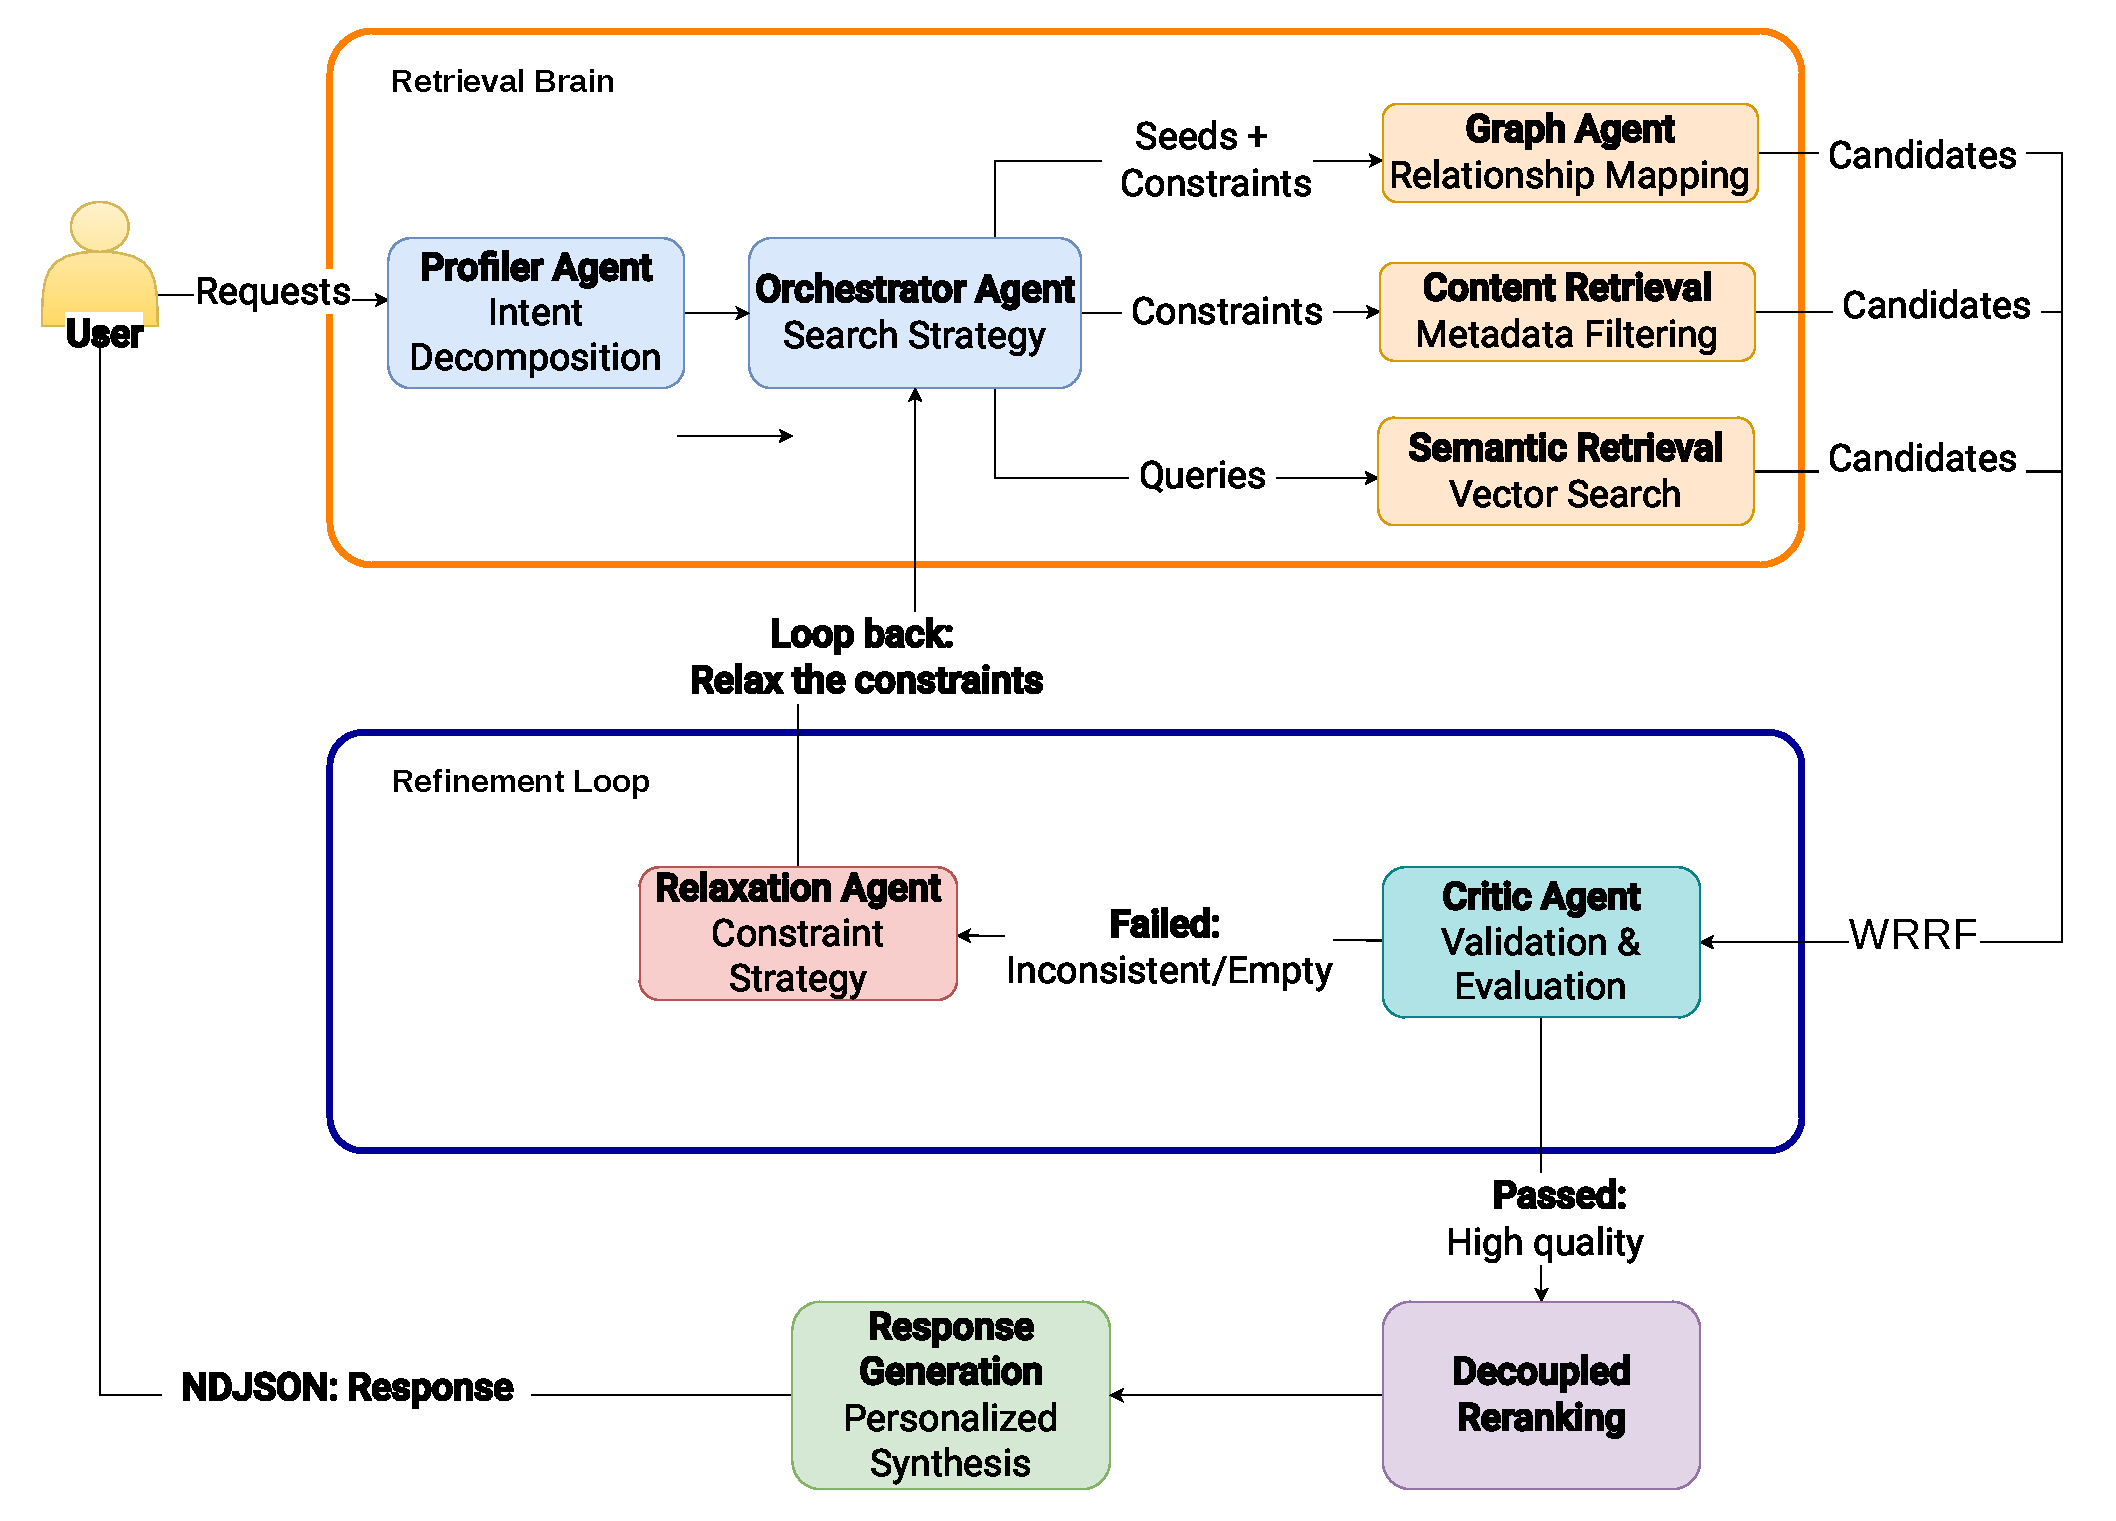
\includegraphics[width=\linewidth]{Chap4/images/argos_architecture.pdf}
    \caption{Kiến trúc tổng quan của hệ thống đa tác tử ARGOS. Khác với kiến trúc tĩnh, ARGOS đưa vào các vòng lặp phản hồi nội bộ (feedback loops) và cơ chế đánh giá lại trọng số động thông qua các Agent chuyên biệt.}
    \label{fig:argos_architecture}
\end{figure}

\section{Tác tử Hồ sơ (Profiler Agent) và Phân rã ý định}

Profiler Agent là tác tử đầu tiên trong chuỗi xử lý, chịu trách nhiệm chuyển hóa yêu cầu ngôn ngữ tự nhiên của người dùng thành các cấu trúc dữ liệu chuẩn hóa (Structured Output) để các tác tử sau có thể sử dụng nhất quán. Quá trình này gồm ba cơ chế cốt lõi, được minh họa tổng quan trong Hình \ref{fig:profiler_agent}.

\begin{figure}[H]
    \centering
    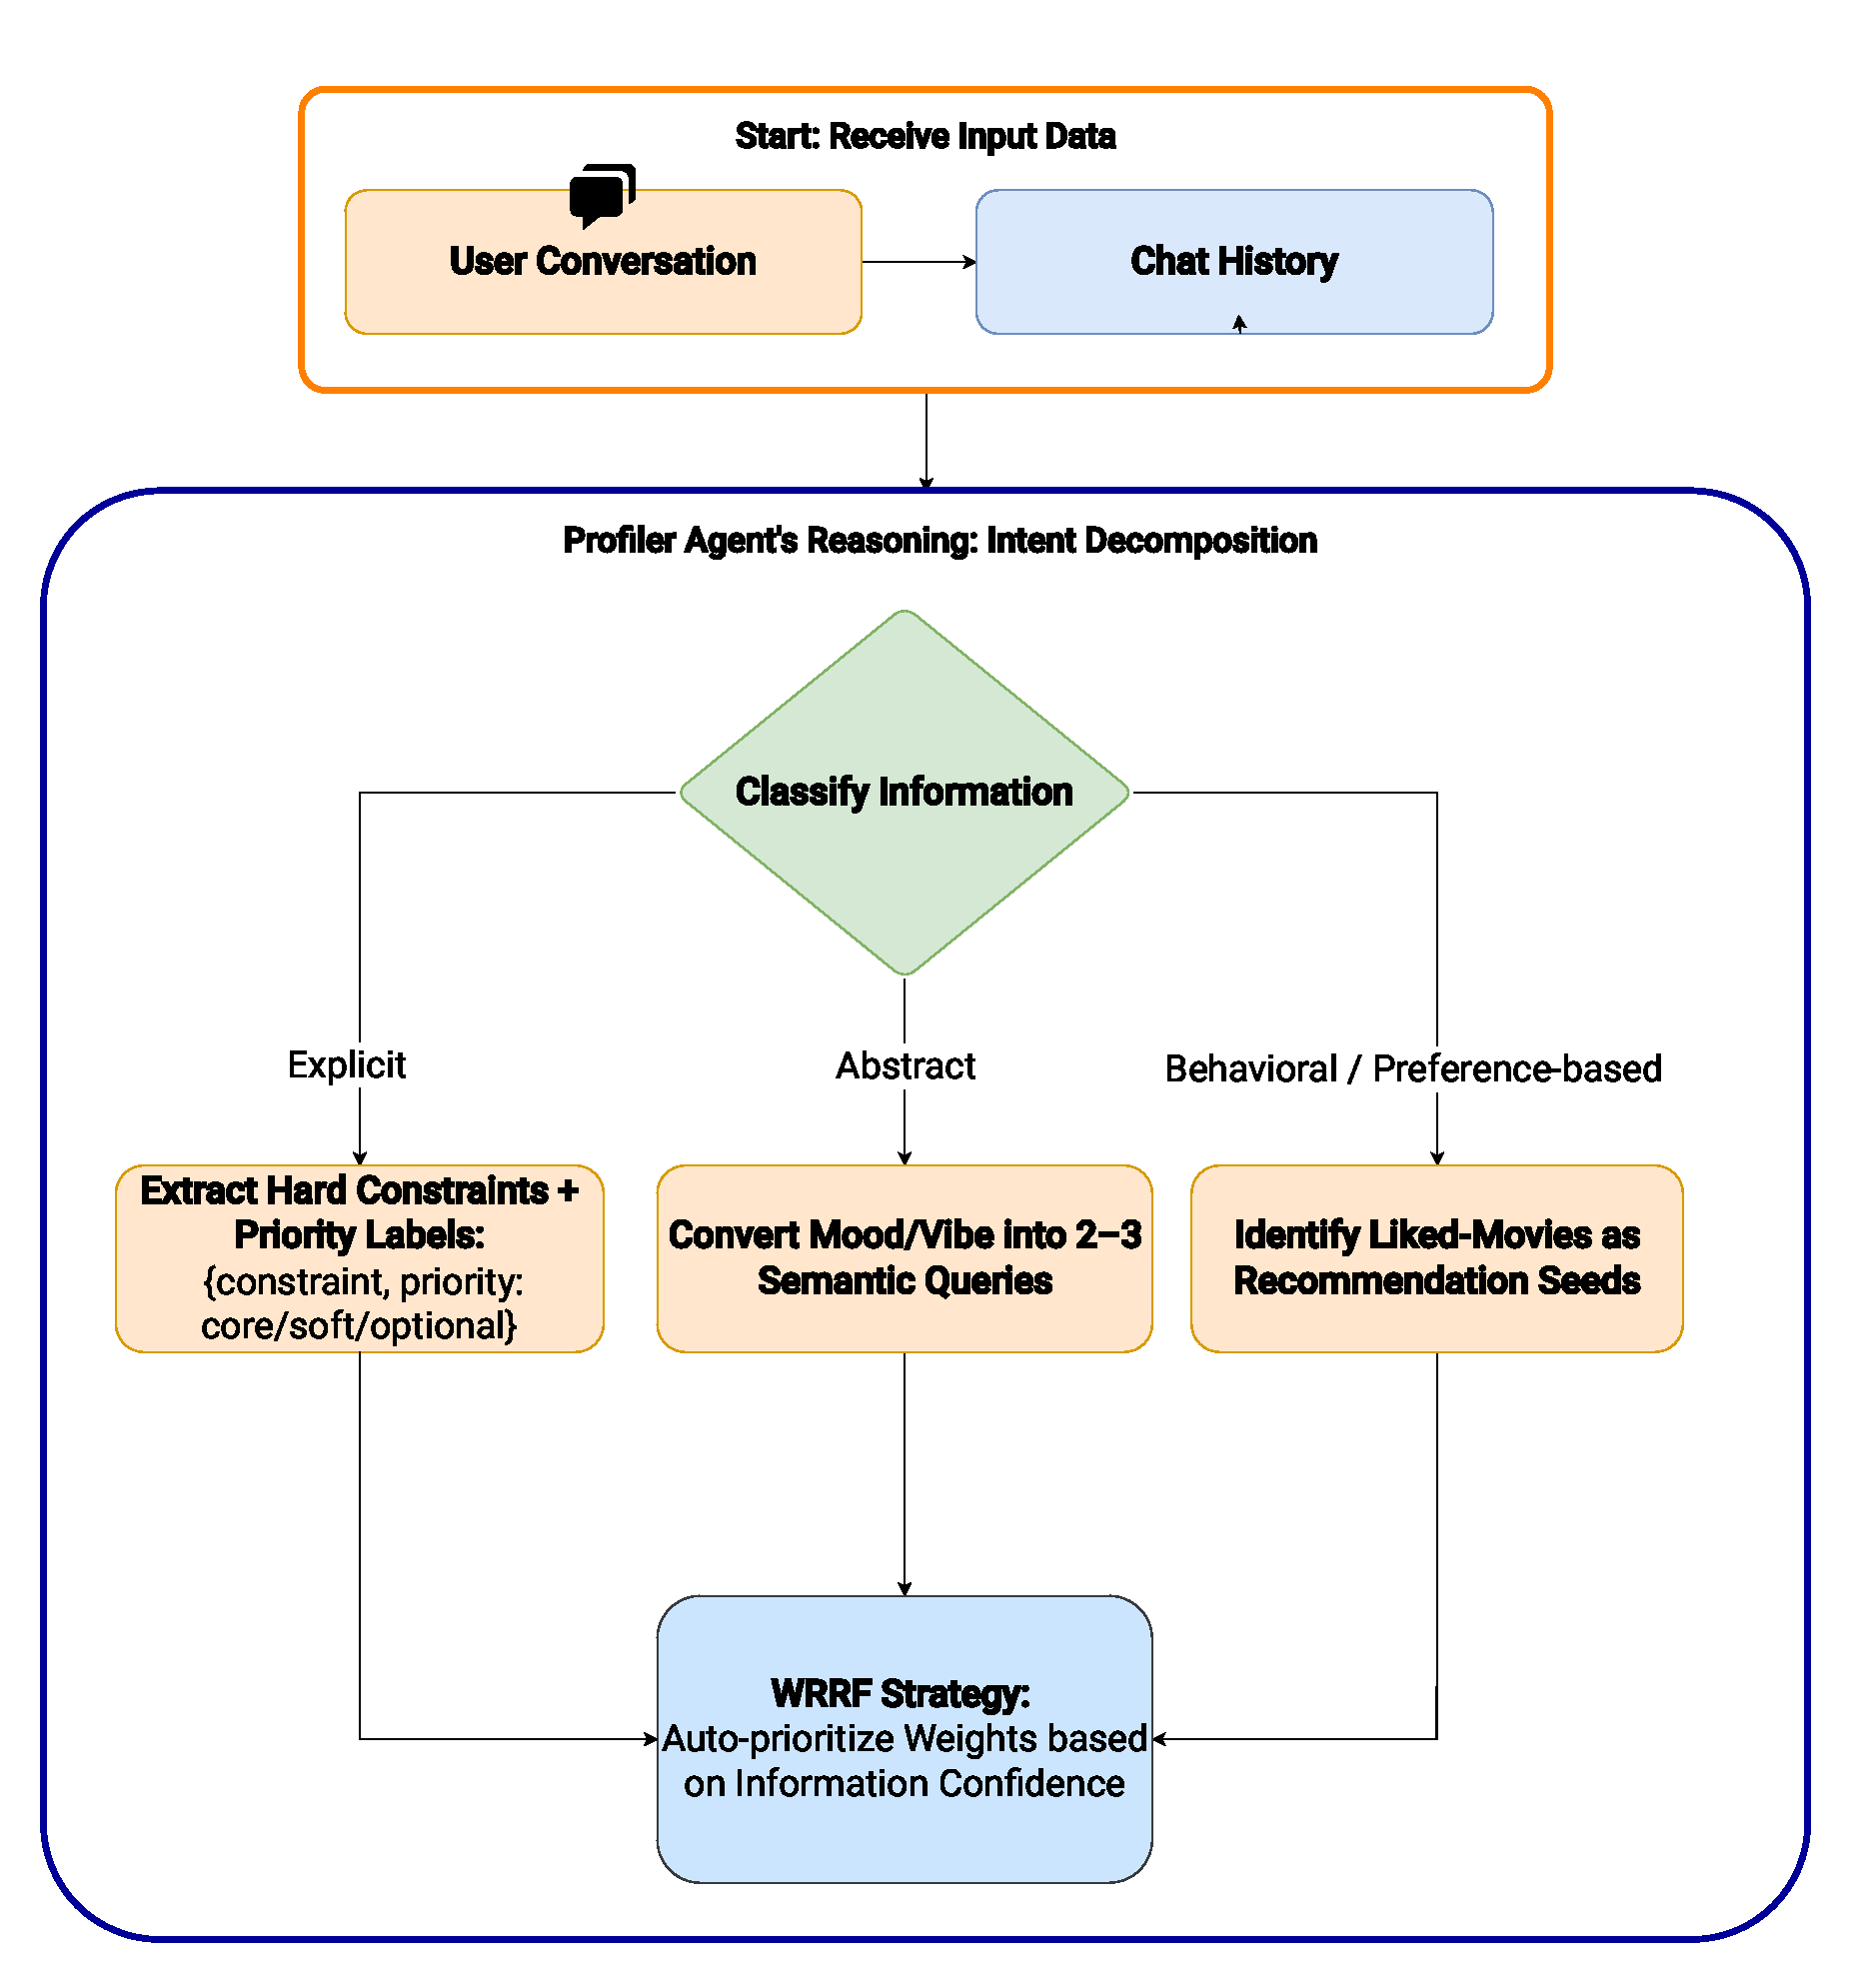
\includegraphics[width=\linewidth]{Chap4/images/profile_agent.pdf}
    \caption{Tổng quan luồng suy luận của Profiler Agent (Intent Decomposition). Từ đầu vào là lượt hội thoại hiện tại và lịch sử chat, tác tử phân loại thông tin thành ba nhánh xử lý độc lập: (1) thông tin \textit{Explicit} được trích xuất thành Ràng buộc cứng (năm, hãng phim, diễn viên); (2) thông tin \textit{Abstract} (cảm xúc, không khí) được chuyển đổi thành 2–3 câu truy vấn ngữ nghĩa; (3) thông tin \textit{Behavioral} (phim đã thích) được xác định làm hạt giống gợi ý (Recommendation Seeds). Ba nhánh hội tụ về bước chiến lược WRRF, nơi trọng số các luồng truy xuất được tự động ưu tiên theo độ tin cậy của từng loại thông tin.}
    \label{fig:profiler_agent}
\end{figure}

Như minh họa trong Hình \ref{fig:profiler_agent}, điểm cốt lõi của Profiler Agent nằm ở bước \textbf{Phân loại thông tin (Classify Information)}: thay vì xử lý đồng nhất toàn bộ phát ngôn người dùng, tác tử nhận diện \textit{bản chất} của từng mảnh thông tin và định tuyến sang pipeline phù hợp. Thông tin tường minh (Explicit) như tên diễn viên, năm phát hành hay hãng sản xuất đi thẳng vào tập Ràng buộc cứng để làm bộ lọc cho Critic Agent ở giai đoạn sau. Thông tin trừu tượng (Abstract) mang tính cảm xúc như "phim buồn" hay "không khí u ám" được diễn giải thành 2–3 câu truy vấn ngữ nghĩa độc lập nhằm khai thác tối đa không gian vector. Thông tin hành vi (Behavioral) — các bộ phim người dùng đã xem và yêu thích — được dùng làm hạt giống cho luồng Collaborative Retrieval. Sau khi cả ba nhánh hoàn tất, Profiler Agent tổng hợp kết quả và xác định bộ trọng số WRRF phù hợp nhất với hình thái truy vấn hiện tại, cung cấp tín hiệu định tuyến cho Orchestrator Agent.

\subsection{Trích xuất thực thể và Ràng buộc cứng (Fact Extraction)}

Nhiệm vụ trọng tâm của Profiler Agent trong giai đoạn này là chuyển hóa các phát ngôn ngôn ngữ tự nhiên vốn có tính đa nghĩa và mơ hồ thành một tập hợp các vị từ logic (logic predicates) xác định. Tác tử tiến hành nhận diện và trích xuất các thông tin định lượng (năm sản xuất, điểm đánh giá) hoặc các thực thể định danh (tên đạo diễn, diễn viên, hãng phim) có độ tin cậy cao từ ngữ cảnh hội thoại hiện tại và lịch sử tương tác.

Quá trình này không chỉ dừng lại ở việc nhận diện thực thể (Entity Recognition) mà còn bao gồm bước chuẩn hóa tri thức (Knowledge Normalization). Profiler Agent đối soát các thực thể thô được trích xuất với lược đồ hệ thống để đảm bảo tính đồng nhất. Các thông tin sau khi chuẩn hóa được hệ thống hóa thành bộ \textbf{Ràng buộc cứng (Hard Constraints)} theo một cấu trúc dữ liệu nghiêm ngặt. Việc sử dụng các mô hình xác thực dữ liệu đảm bảo rằng mọi đầu ra của LLM đều phải tuân thủ một lược đồ JSON (JSON Schema) tiền định, triệt tiêu các sai số về định dạng trong quá trình truyền tin giữa các tác tử. Một ví dụ về cấu trúc ràng buộc cứng được minh họa như sau:

\begin{verbatim}
{
  "genres": ["Action", "Sci-Fi"],
  "directors": ["Christopher Nolan"],
  "release_year_range": [2010, 2020],
  "forbidden_elements": ["Romance"],
  "min_rating": 8.0
}
\end{verbatim}

Điểm khác biệt quan trọng của ARGOS so với các hệ thống RAG thông thường nằm ở vai trò của bộ hồ sơ này. Các ràng buộc cứng đóng vai trò là tiêu chí kiểm định bắt buộc. Trong các khâu kiểm định hậu kỳ (Critic phase), bất kỳ vật phẩm gợi ý nào không thỏa mãn dù chỉ một tiêu chí trong danh sách trên (ví dụ: phim thuộc thể loại Romance dù người dùng đã cấm) sẽ bị loại bỏ ngay lập tức khỏi tập kết quả. Cơ chế này đóng vai trò như một bộ lọc tiền định, bảo vệ hệ thống khỏi các lỗi ảo giác ngữ nghĩa của mô hình ngôn ngữ ở các giai đoạn sau.

Song song với việc trích xuất ràng buộc cứng từ thông tin tường minh, Profiler Agent còn xử lý nhánh thứ ba trong sơ đồ phân loại: thông tin hành vi (Behavioral). Cụ thể, các bộ phim người dùng đã đề cập tích cực trong lịch sử hội thoại (ví dụ: \textit{"tôi rất thích John Wick"}) được nhận diện và đánh dấu là \textbf{hạt giống gợi ý (Recommendation Seeds)}. Tập hạt giống này được chuyển trực tiếp đến Orchestrator Agent để khởi động luồng Collaborative Retrieval — duyệt Đồ thị tri thức để tìm các phim có chung diễn viên, đạo diễn hoặc ekip sáng tạo với các hạt giống đó.


\subsection{Đa dạng hóa ngữ nghĩa (Intent Expansion / Multi-Query)}
Trong các mô hình truy xuất ngữ nghĩa (Dense Retrieval) truyền thống, việc mã hóa toàn bộ truy vấn phức tạp của người dùng vào một vector duy nhất (single embedding vector) thường dẫn đến hiện tượng "sụp đổ ngữ nghĩa" (semantic collapse). Khi một câu lệnh chứa nhiều khái niệm trực giao (orthogonal concepts), không gian vector thường phải lấy trung bình (average out), làm phai nhòa các đặc trưng quan trọng.

Để khắc phục hạn chế này, Profiler Agent triển khai chiến lược \textbf{đa truy vấn (Multi-Query Expansion)}. Thay vì chỉ sử dụng một biểu diễn chung, tác tử phân rã ý định ban đầu thành một tập hợp các góc độ truy vấn độc lập $Q = \{q_1, q_2, \dots, q_n\}$. Các câu truy vấn này khai thác các đặc trưng tiềm ẩn (latent semantic features) riêng biệt như:
\begin{itemize}
    \item \textbf{Cốt truyện và Chủ đề (Plot \& Theme):} Trích xuất nội dung lõi của câu chuyện.
    \item \textbf{Không khí và Cảm xúc (Vibe \& Mood):} Trích xuất sắc thái cảm nhận mà người dùng mong muốn.
    \item \textbf{Bối cảnh và Kỹ thuật điện ảnh (Setting \& Cinematography):} Các yếu tố về hình ảnh, thời đại hoặc phong cách.
\end{itemize}
Điển hình, một yêu cầu phức tạp như "Tôi muốn xem một phim giống John Wick, bối cảnh Châu Á nhưng mang màu sắc buồn bã" sẽ không bị nén thành một vector hỗn độn. Thay vì đó, Profiler phân giải nó thành: $q_1 =$ "hành động nhịp độ cao, sát thủ", $q_2 =$ "bối cảnh Nhật Bản hoặc Hồng Kông", và $q_3 =$ "tâm lý nặng nề, kết cục bi thảm".

Quá trình này giúp mở rộng không gian tìm kiếm đa chiều (multi-dimensional search space), gia tăng đáng kể tỷ lệ bao phủ (Recall) của hệ thống. Cần lưu ý rằng, mặc dù việc phân rã ý định có vẻ giống một phép toán hợp (OR) tại bước truy xuất để tối ưu độ phủ, tính hội tụ và điều kiện giao (AND) của các yêu cầu vẫn được đảm bảo chặt chẽ ở các giai đoạn sau thông qua thuật toán hợp nhất thứ hạng (Fusion) và bước đối soát của Critic Agent.

\subsection{Dự báo chiến lược trọng số động (Dynamic Weighting / Adaptive Routing)}
Trong kiến trúc tĩnh GRACE, việc hợp nhất kết quả từ nhiều luồng dữ liệu (Semantic, Content, Graph) phụ thuộc vào một bộ siêu tham số (hyperparameters) tĩnh. Tuy nhiên, mỗi truy vấn lại yêu cầu một cấu hình khác nhau. Ví dụ, câu hỏi "Phim nào của Christopher Nolan đạo diễn?" mang đậm tính cấu trúc, trong khi câu "Phim nào khiến tôi phải suy ngẫm về nhân sinh?" lại mang đậm tính ngữ nghĩa.

Sau khi hoàn tất bước phân loại thông tin, Profiler Agent tổng hợp kết quả từ cả ba nhánh để xác định bộ trọng số WRRF phù hợp. Nguyên tắc cốt lõi là \textbf{ưu tiên trọng số theo độ tin cậy của thông tin (Information Confidence)}: nhánh nào trích xuất được nhiều thông tin chất lượng cao thì luồng truy xuất tương ứng được khuếch đại. Dựa trên đó, Profiler Agent dự báo một vector phân bố trọng số $\mathbf{w}(C)$ cho các luồng truy xuất theo ngữ cảnh hội thoại $C$:
\begin{equation}
    \mathbf{w}(C) = (w_{\text{sem}}, w_{\text{con}}, w_{\text{col}})^T, \quad \text{với} \quad \sum_{i \in \{\text{sem, con, col}\}} w_i = 1, \quad w_i \in [0, 1]
\end{equation}
Trong đó:
\begin{itemize}
    \item $w_{\text{sem}}$ (Trọng số Ngữ nghĩa - Semantic Weight): Tăng cao khi truy vấn chứa nhiều tính từ mô tả, cảm xúc, hoặc so sánh tương đồng ("giống phim A nhưng buồn hơn").
    \item $w_{\text{con}}$ (Trọng số Nội dung - Content Weight): Được ưu tiên khi người dùng chỉ định rõ các tiêu chí lọc cứng như thể loại, khoảng năm phát hành, hoặc ngưỡng điểm đánh giá (IMDb/Rating).
    \item $w_{\text{col}}$ (Trọng số Đồ thị - Graph Weight): Được kích hoạt khi truy vấn chỉ định rõ các thực thể danh định (Entities) như tên diễn viên, đạo diễn, hãng phim, hoặc khi cần khai thác lịch sử hồ sơ người dùng (User Profile) để mở rộng tìm kiếm.
\end{itemize}
Việc định tuyến linh hoạt (Adaptive Routing) này giúp ARGOS tự động điều phối tài nguyên tìm kiếm, tối ưu hóa sự kết hợp của nhiều nguồn tri thức mà không cần sự can thiệp thủ công của kỹ sư vào mã nguồn. Cơ chế này được minh họa cụ thể trong Hình \ref{fig:adaptive_weighting}.

\begin{figure}[H]
    \centering
    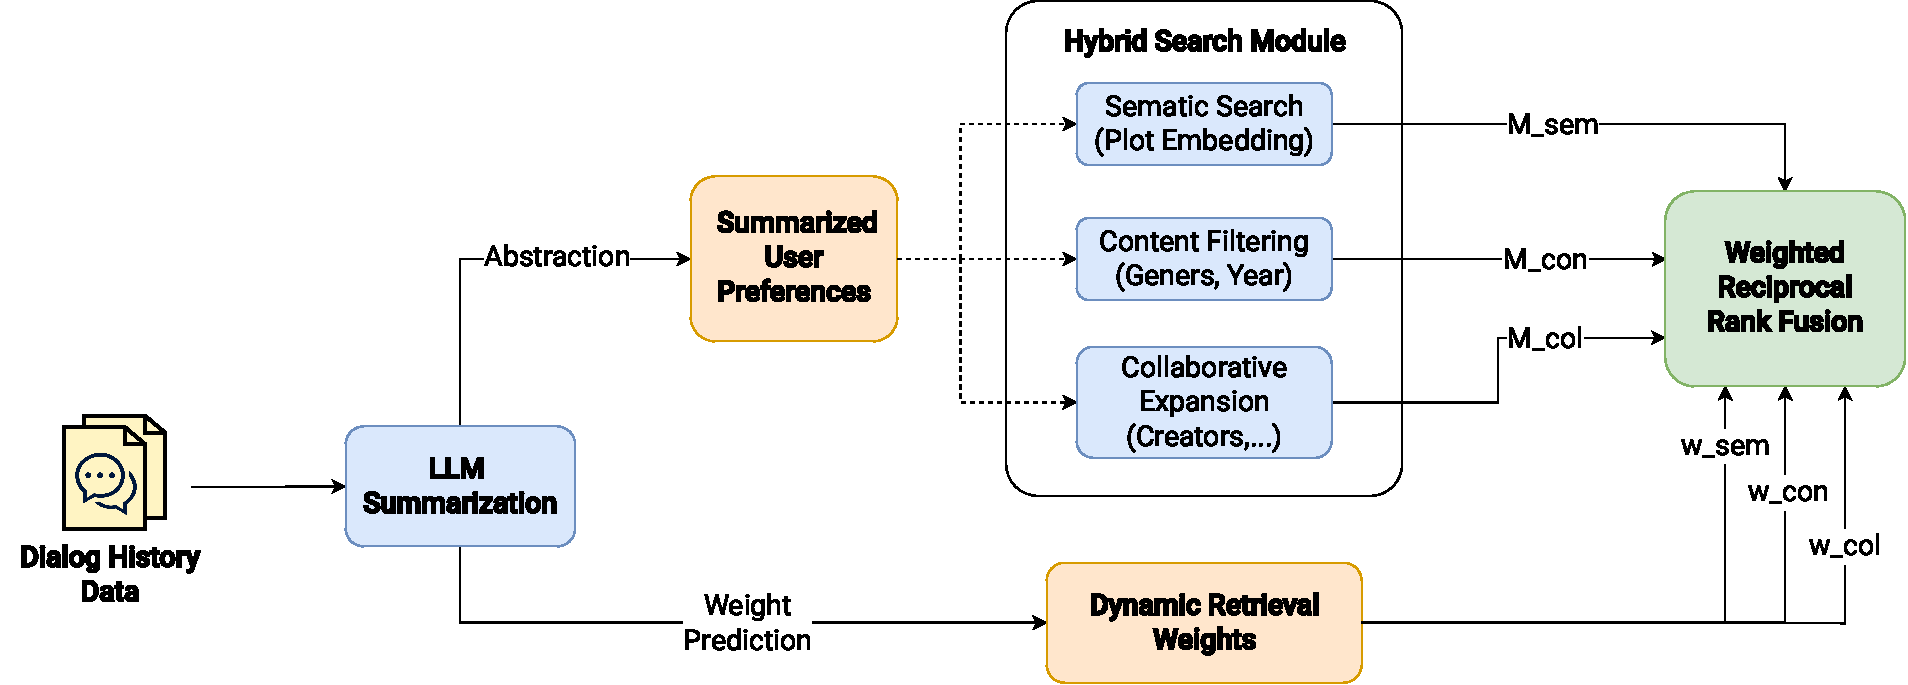
\includegraphics[width=\linewidth]{Chap4/images/adaptive_weighting.pdf}
    \caption{Cơ chế dự báo trọng số động (Dynamic Weight Prediction) do Profiler Agent thực hiện, cung cấp tín hiệu định tuyến cho các luồng truy xuất.}
    \label{fig:adaptive_weighting}
\end{figure}

\section{Tác tử Đồ thị (Graph Agent) với Vòng lặp ReAct}

Tác tử Đồ thị có nhiệm vụ tương tác trực tiếp với cơ sở dữ liệu đồ thị, khai thác cấu trúc đồ thị đa quan hệ (multi-relational graph structure) để định vị các thực thể thông qua các bước nhảy logic (multi-hop reasoning).

\subsection{Nhận thức cấu trúc dữ liệu (Schema-Aware Intelligence)}
Điểm yếu thường thấy khi giao tiếp tự do giữa LLM và cơ sở dữ liệu đồ thị là LLM có xu hướng "ảo giác" ra các nút (nodes) hoặc các mối quan hệ (edges) không hề tồn tại trong cơ sở dữ liệu thực tế. Ví dụ, LLM có thể sinh ra các câu truy vấn đồ thị sai lệch về cấu trúc nút, trong khi đồ thị thực tế chỉ cho phép những liên kết nhất định giữa các thực thể (như Người dùng thich Phim thay vì Người dùng thích Diễn viên). 

Để giải quyết vấn đề này, Graph Agent được trang bị cơ chế \textbf{Nhận thức cấu trúc dữ liệu (Schema-Aware Intelligence)}. Hệ thống liên tục cung cấp cho tác tử một siêu dữ liệu (metadata snapshot) chứa danh sách các nhãn (Labels) và các loại quan hệ (Relationships) hợp lệ. Nhờ sự ràng buộc khắt khe này, tác tử có thể ánh xạ chính xác các nhu cầu trừu tượng của người dùng vào không gian đồ thị. Đồng thời, tác tử được tích hợp khả năng khai thác các phương pháp truy vấn liên kết, cho phép đối chiếu danh sách các phim người dùng đã thích để nội suy các kết nối ẩn về diễn viên hoặc đạo diễn một cách an toàn.

\subsection{Vòng lặp Suy luận và Hành động (Reasoning + Acting)}
Đặc điểm cốt lõi tạo nên sự khác biệt của Graph Agent là việc tích hợp mô hình suy luận ReAct (Reasoning and Acting) \cite{yao2022react}. Khác với các hệ thống chuyển đổi ngôn ngữ sang truy vấn đồ thị (Text-to-Graph Query) thụ động, tác tử vận hành dựa trên một chuỗi các trạng thái động được định nghĩa hình thức tại bước $t$ như sau:
\begin{equation}
    \text{Thought}_t \rightarrow \text{Action}_t (\text{Graph Query}) \rightarrow \text{Observation}_t (\text{DB Result})
\end{equation}

Trong chu trình tối đa 3 lượt (turns), hệ thống tiến hành các bước:
\begin{enumerate}
    \item \textbf{Action:} Tác tử sinh mã truy vấn đồ thị dựa trên ý định đầu vào và sơ đồ cấu trúc.
    \item \textbf{Observation:} Khác biệt với các hệ thống tĩnh thường sụp đổ khi gặp lỗi biên dịch (compile error), Graph Agent thu nhận trực tiếp thông báo lỗi từ hệ quản trị cơ sở dữ liệu hoặc nhận về một danh sách kết quả rỗng (empty list).
    \item \textbf{Thought:} Dựa trên Observation, tác tử tự phân tích nguyên nhân sự cố. Nó nhận thức được rằng trường dữ liệu \texttt{'studio'} bị thiếu và tự động đề xuất giải pháp thay thế, chẳng hạn như chuyển sang tìm kiếm dựa trên \texttt{'production\_company'}.
\end{enumerate}
Cơ chế tự sửa lỗi (Self-Correction) này giúp hệ thống xử lý được các tình huống sai lệch cấu trúc đồ thị (Schema Mismatch) mà không cần lập trình viên viết thêm logic xử lý ngoại lệ cho từng trường hợp cụ thể. Quy trình này được mô phỏng chi tiết trong Hình \ref{fig:graph_agent_react}.


\begin{figure}[H]
    \centering
    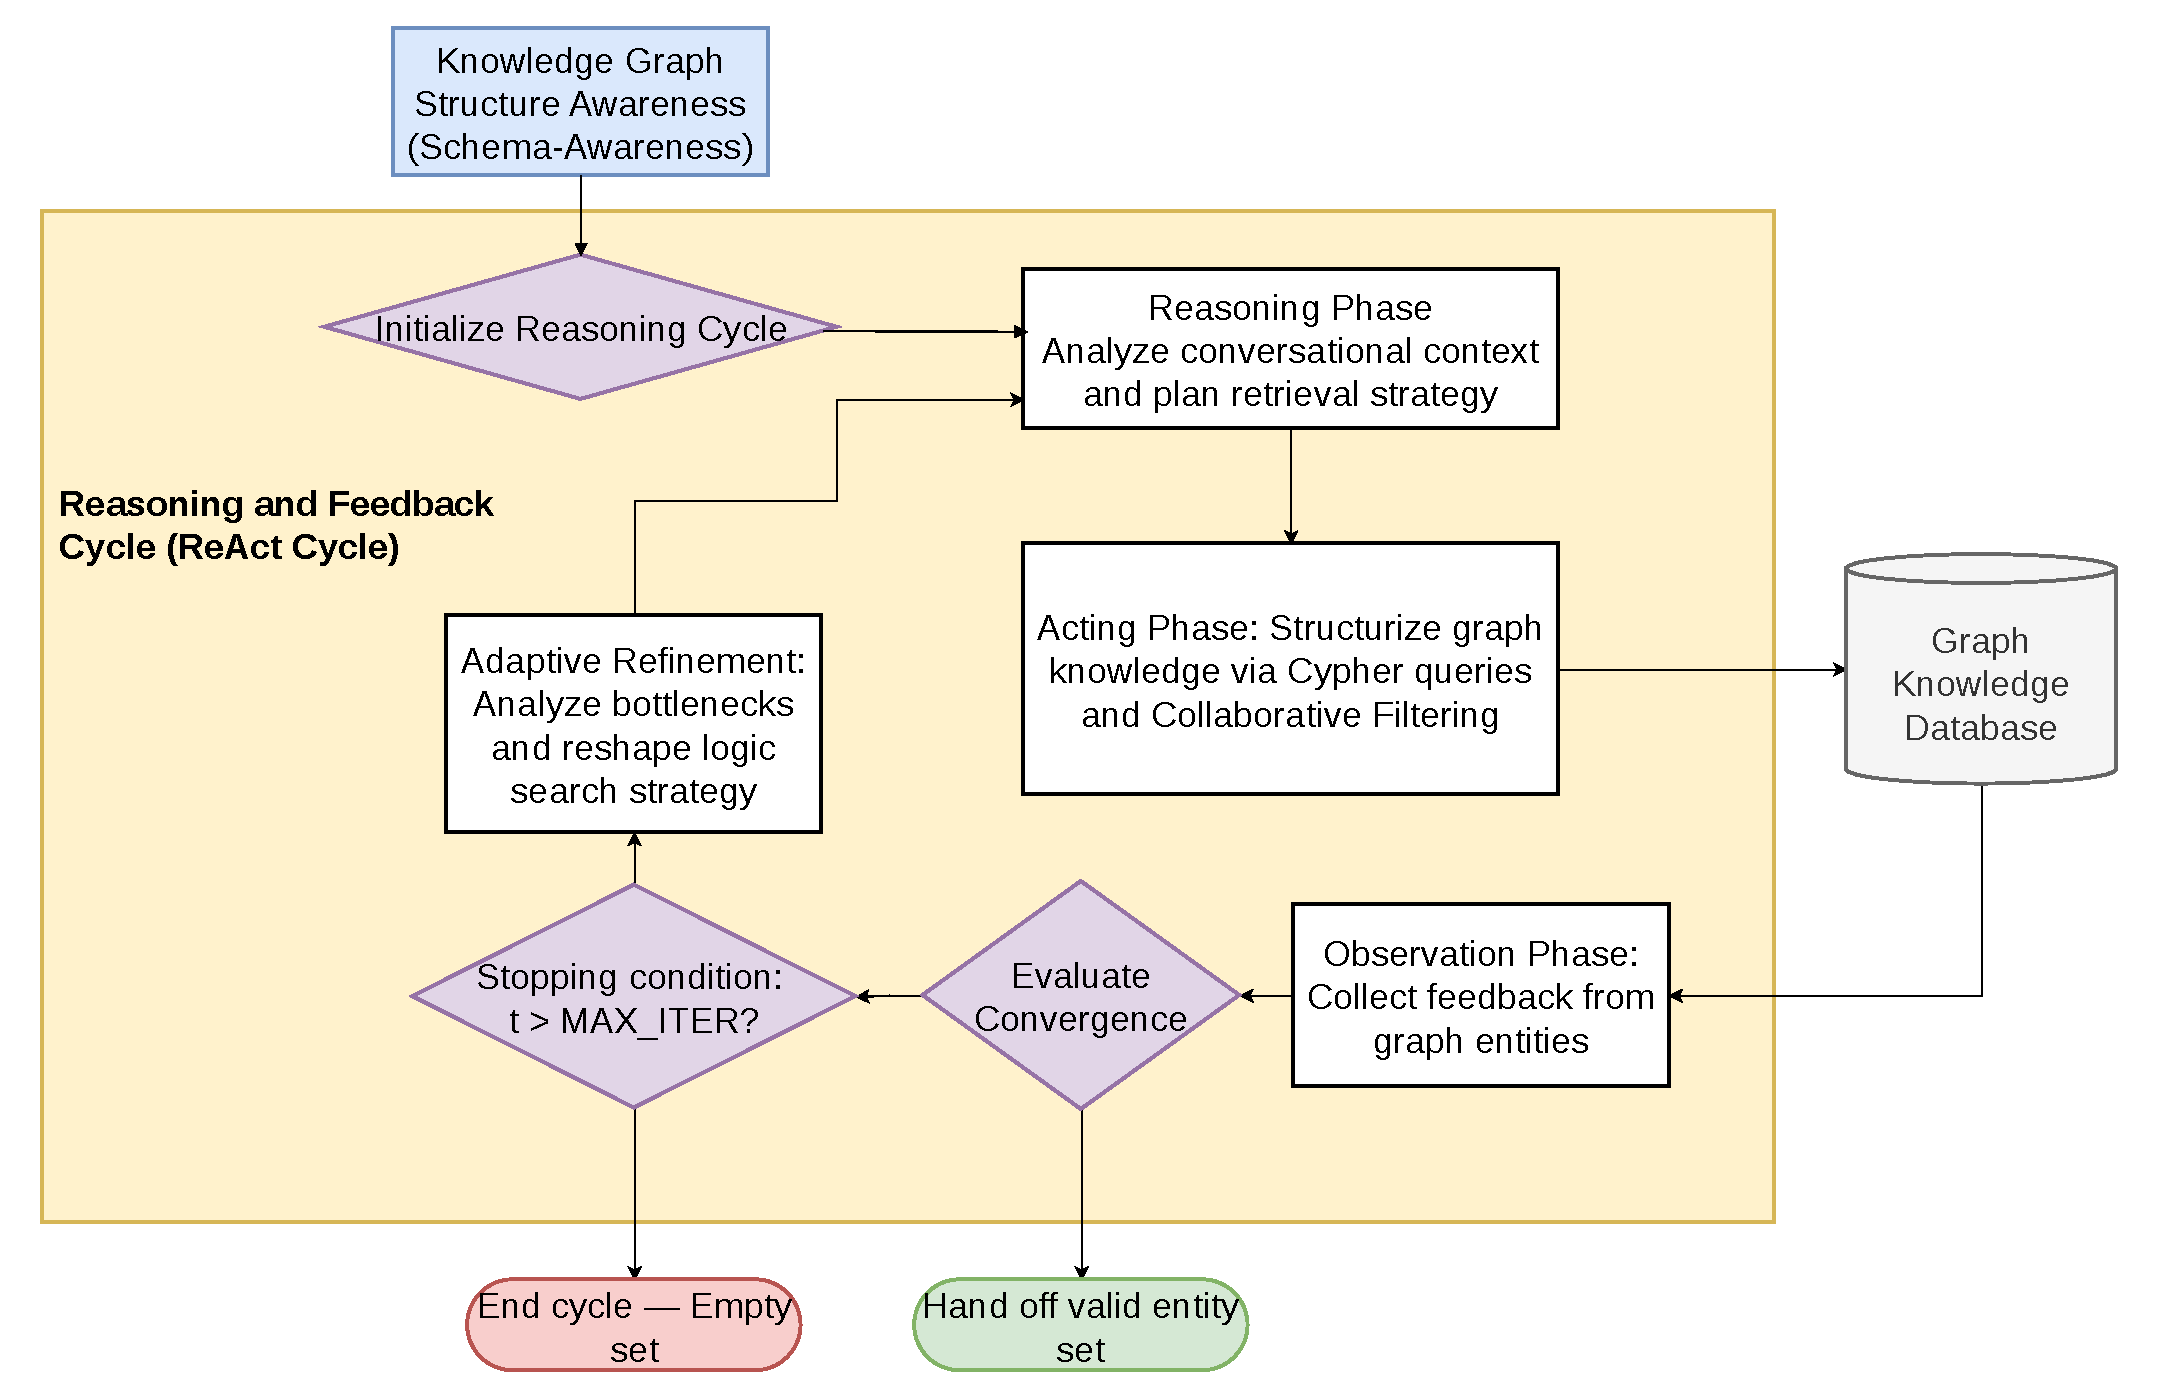
\includegraphics[width=\linewidth]{Chap4/images/graph_agent.pdf}
    \caption{Sơ đồ chu trình suy luận và phản hồi (ReAct Cycle) của Graph Agent. Dựa trên nhận thức về cấu trúc đồ thị (Schema-Awareness), hệ thống tiến hành vòng lặp Suy luận - Hành động - Quan sát, kết hợp cơ chế đánh giá tính hội tụ và tự thích nghi (Refinement) để tối ưu chiến lược truy vấn.}
    \label{fig:graph_agent_react}
\end{figure}

\section{Trung tâm Điều phối (Orchestrator Agent)}

Orchestrator Agent hoạt động như một module điều phối trung tâm, chịu trách nhiệm quản lý tài nguyên và tổng hợp thứ hạng. Hình \ref{fig:orchestrator_strategy} minh họa luồng tư duy và chiến lược tìm kiếm đa luồng của Orchestrator.

\begin{figure}[H]
    \centering
    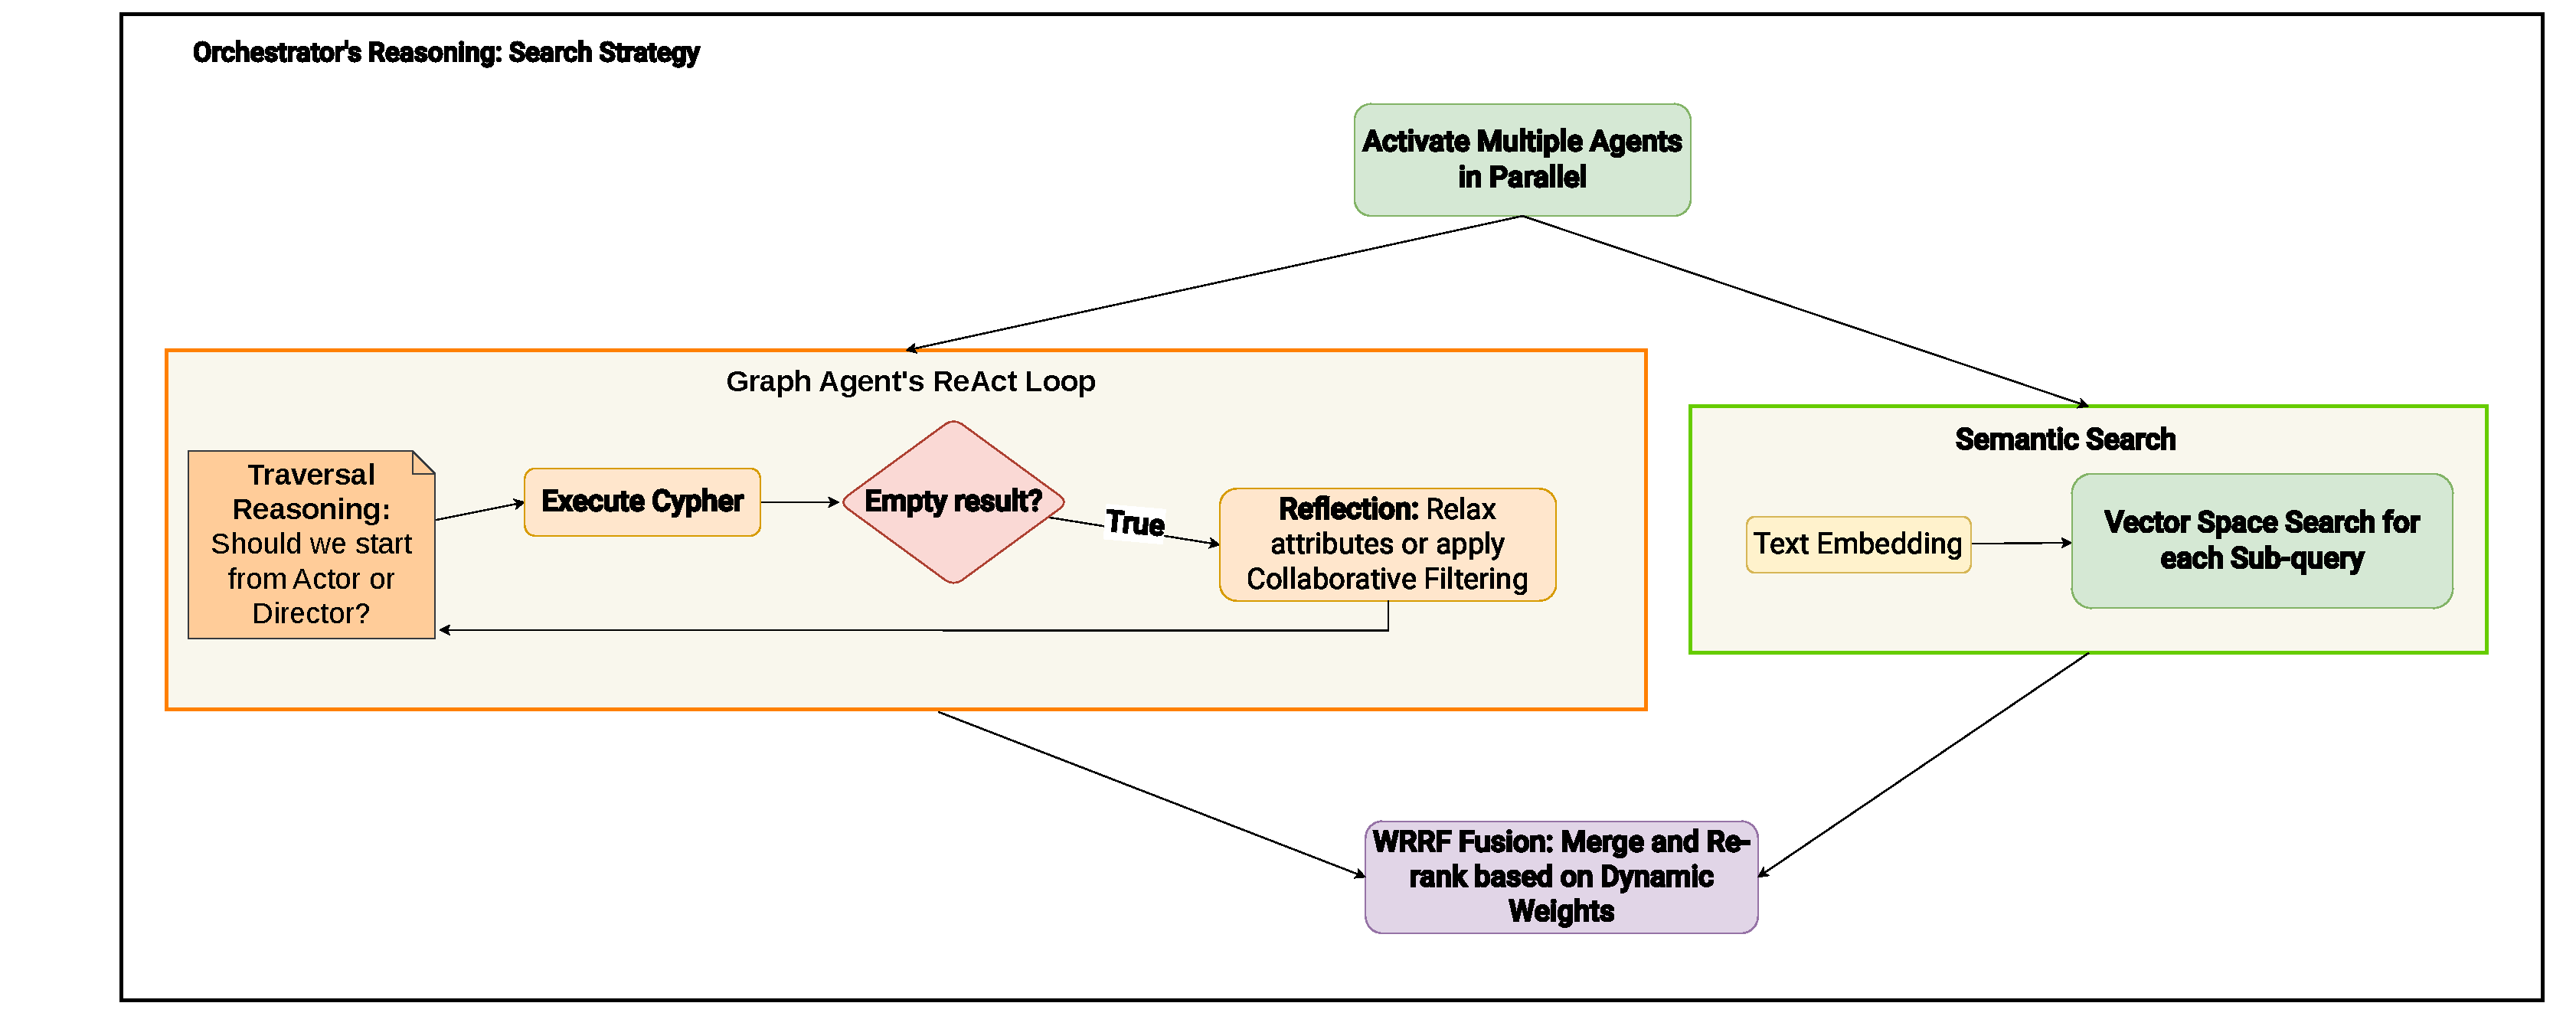
\includegraphics[width=\linewidth]{Chap4/images/Orchestrator.pdf}
    \caption{Chiến lược tìm kiếm đa luồng của Orchestrator Agent. Hệ thống kích hoạt song song Vòng lặp ReAct của Graph Agent và Tìm kiếm Ngữ nghĩa (Semantic Search), sau đó hợp nhất kết quả thông qua thuật toán WRRF Fusion có sử dụng trọng số động.}
    \label{fig:orchestrator_strategy}
\end{figure}

\subsection{Thực thi truy xuất bất đồng bộ (Asynchronous Parallel Execution)}
Khác với mô hình đường ống tuần tự (sequential pipeline), Orchestrator được thiết kế để tối thiểu hóa độ trễ (latency) thông qua kiến trúc lập trình bất đồng bộ (asynchronous programming). Ngay khi Profiler Agent hoàn tất việc phân rã ý định, Orchestrator sẽ kích hoạt đồng thời ba luồng truy xuất độc lập:
\begin{itemize}
    \item \textbf{Semantic Retrieval:} Tìm kiếm trên không gian vector mật độ cao (Dense Vector DB) để nắm bắt ý nghĩa tiềm ẩn.
    \item \textbf{Content Retrieval:} Khớp lệnh chính xác (Exact Match) trên cơ sở dữ liệu quan hệ hoặc hệ thống tìm kiếm văn bản để lọc theo các siêu dữ liệu cứng (metadata).
    \item \textbf{Graph Retrieval:} Thực thi vòng lặp ReAct của Graph Agent trên cơ sở dữ liệu đồ thị để tìm kiếm các thực thể liên kết đa bước.
\end{itemize}
Quá trình xử lý song song này đảm bảo hệ thống có thể quét qua toàn bộ mặt phẳng dữ liệu khổng lồ mà không làm tăng thời gian phản hồi tổng thể (Time-To-First-Token). Điểm nghẽn về tốc độ sẽ chỉ phụ thuộc vào luồng phản hồi chậm nhất (thường là Graph Agent), thay vì tổng thời gian của cả ba luồng cộng lại.

\subsection{Hợp nhất thứ hạng với thuật toán WRRF (Dynamic WRRF)}
Mỗi luồng truy xuất sẽ trả về một danh sách các ứng viên độc lập với thang điểm (score scale) hoàn toàn khác nhau (ví dụ: điểm Cosine Similarity của cơ sở dữ liệu Vector khác biệt hoàn toàn với điểm số cấu trúc của đồ thị). Để đồng bộ hóa, Orchestrator áp dụng thuật toán Hợp nhất Thứ hạng Nghịch đảo có Trọng số (Weighted Reciprocal Rank Fusion - WRRF).

Cho $R_m(i)$ là thứ hạng của vật phẩm $i$ trong danh sách trả về của phương pháp truy xuất $m \in \{\text{sem, con, col}\}$, điểm số cuối cùng của vật phẩm $i$ được tính bằng:
\begin{equation}
    \text{WRRF\_Score}(i) = \sum_{m} \frac{w_m}{k + R_m(i)}
\end{equation}
Trong đó:
\begin{itemize}
    \item $w_m$ là trọng số của phương pháp $m$ do Profiler Agent dự báo theo ngữ cảnh hội thoại tại mỗi lượt. Đây là khác biệt cốt lõi so với GRACE, nơi bộ trọng số được cố định tại $(w_{\text{sem}}, w_{\text{con}}, w_{\text{col}}) = (0.40, 0.35, 0.25)$ cho toàn bộ hệ thống.
    \item $k$ là một hằng số làm mượt (smoothing constant), thường được đặt bằng 60 để ngăn chặn các vật phẩm ở top 1 chiếm ưu thế quá mức.
\end{itemize}
Cơ chế WRRF vinh danh các ứng viên xuất hiện ở phần giao tập hợp (intersection) của nhiều phương pháp tìm kiếm (nghĩa là vừa có ngữ nghĩa tốt, vừa có liên kết đồ thị mạnh). Điều này giải quyết bài toán "điều kiện hợp" (OR) của Multi-Query: một vật phẩm chỉ thỏa mãn $q_1$ sẽ có thứ hạng thấp hơn nhiều so với vật phẩm thỏa mãn đồng thời cả $\{q_1, q_2, q_3\}$. Do đó, WRRF đóng vai trò như một phép toán "giao mềm" (soft AND), định hướng sự hội tụ về phía các kết quả thỏa mãn toàn diện ý định người dùng. Việc áp dụng trọng số động $w_m$ giúp khuếch đại ảnh hưởng của luồng dữ liệu phù hợp nhất với loại truy vấn, từ đó tạo ra một danh sách ứng viên ưu tú mang tính thích ứng cao để chuyển giao cho pha kiểm định.

\section{Tác tử Kiểm định (Critic Agent) - Kiểm soát chất lượng}

Tác tử kiểm định (Critic Agent) đóng vai trò là một cơ chế rà soát độc lập (Quality Gate) trong kiến trúc ARGOS, hoạt động như một đối trọng để kiểm soát tính hợp lệ của danh sách ứng viên do các module truy xuất cung cấp. Cơ chế hoạt động của Critic Agent được minh họa trong Hình \ref{fig:critic_agent}.


\begin{figure}[H]
    \centering
    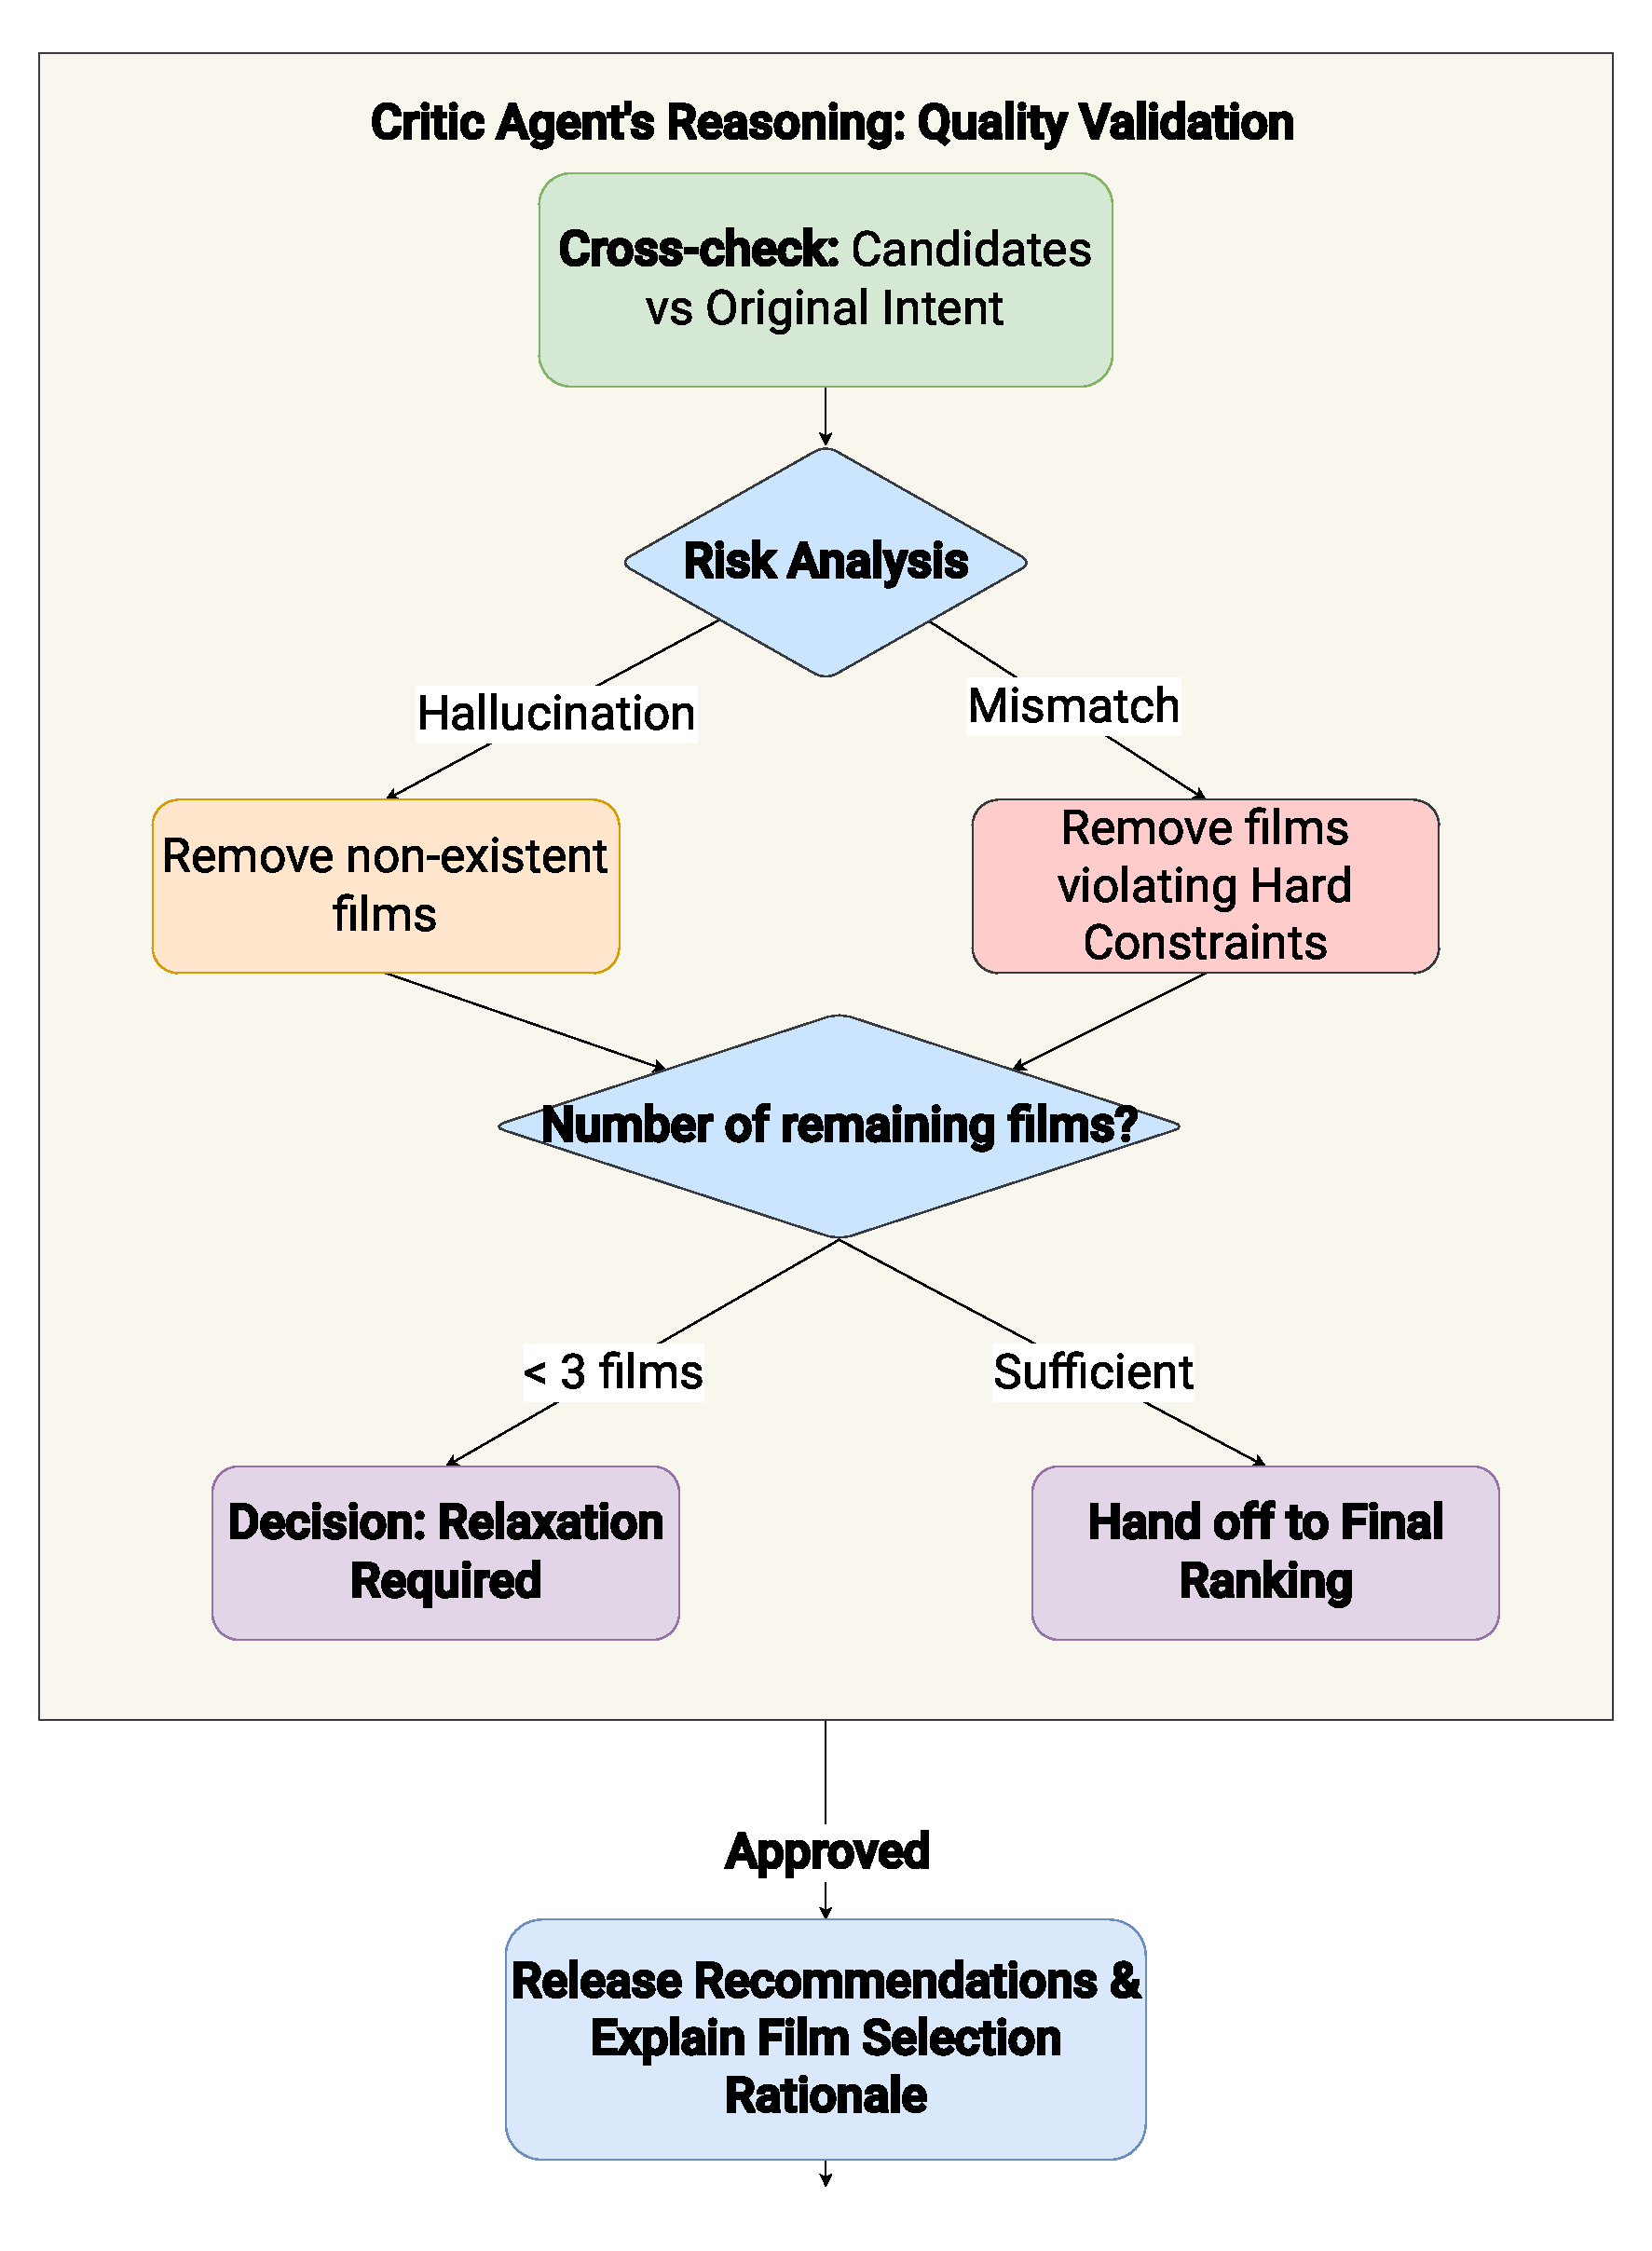
\includegraphics[width=\linewidth]{Chap4/images/critic_agent.pdf}
    \caption{Cơ chế hoạt động của Critic Agent. Tác tử thực hiện đối soát chéo các ứng viên với Ràng buộc cứng (Hard Constraints) và kích hoạt cơ chế phản hồi (Feedback Trigger) nếu số lượng ứng viên hợp lệ không đạt ngưỡng dung sai.}
    \label{fig:critic_agent}
\end{figure}

\subsection{Đối soát chéo và triệt tiêu ảo giác (Anti-Hallucination)}
Trong hệ thống RAG tĩnh, nếu LLM tự "bịa" ra một bộ phim không tồn tại (Fact Confabulation) hoặc đưa ra một phim không khớp với ràng buộc thời gian (Temporal Inconsistency), hệ thống thường chấp nhận và trả về trực tiếp cho người dùng. Điều này làm suy giảm nghiêm trọng độ tin cậy.

Danh sách ứng viên thu thập được từ Orchestrator sẽ trải qua quá trình đối soát nghiêm ngặt bởi Critic Agent. Tác tử thực hiện ánh xạ và so sánh trực tiếp các thuộc tính siêu dữ liệu (metadata) thực tế của từng ứng viên với tập hợp Ràng buộc cứng (Hard Constraints) đã được trích xuất ở pha Profiler. Quá trình này áp dụng logic Boolean chặt chẽ:
\begin{itemize}
    \item \textbf{Xác thực thực thể (Entity Verification):} Kiểm tra xem ID phim có thực sự tồn tại trong cơ sở dữ liệu hay không, loại bỏ hoàn toàn các phim do LLM tưởng tượng ra.
    \item \textbf{Kiểm tra ràng buộc loại trừ (Exclusion Check):} Đảm bảo không có bộ phim nào chứa các nhãn (tags) nằm trong danh sách \texttt{forbidden\_elements}.
    \item \textbf{Đánh giá ngưỡng (Thresholding):} Lọc bỏ các phim có điểm đánh giá (rating) thấp hơn \texttt{min\_rating} do người dùng quy định.
\end{itemize}
Những thực thể vi phạm bất kỳ ràng buộc logic nào sẽ bị loại bỏ không khoan nhượng nhằm bảo toàn chỉ số độ chuẩn xác (Precision) tuyệt đối của hệ thống.

\subsection{Kích hoạt phản hồi và Lập báo cáo lỗi (Feedback Trigger \& Error Reporting)}
Sau khi sàng lọc qua bộ Ràng buộc cứng, hệ thống thu được tập hợp ứng viên hợp lệ $M_{\text{valid}}$. Critic Agent thực hiện kiểm tra điều kiện ngắt quãng dựa trên ngưỡng dung sai $\tau$ (thường thiết lập $\tau = 1$ để đảm bảo ít nhất luôn có 1 kết quả trả về):
\begin{equation}
    \text{Trigger} =
    \begin{cases}
        \text{Accept},               & \text{nếu } |M_{\text{valid}}| \ge \tau \\
        \text{Relaxation\_Required}, & \text{nếu } |M_{\text{valid}}| < \tau
    \end{cases}
\end{equation}

Nếu tín hiệu \texttt{Relaxation\_Required} được phát ra, thay vì chỉ trả về trạng thái thất bại tĩnh (như mã lỗi 404), Critic Agent sẽ đóng vai trò như một kỹ sư kiểm thử (QA Engineer). Nó sẽ tổng hợp một báo cáo phân tích lỗi (Error Report) bằng ngôn ngữ tự nhiên hoặc JSON, chỉ rõ \textit{chính xác ràng buộc nào đã bị vi phạm}. Ví dụ: \textit{"Tìm thấy 5 phim hành động của đạo diễn Nolan, nhưng không có phim nào phát hành sau năm 2020 như yêu cầu."} Báo cáo này là cơ sở dữ liệu đầu vào mang tính sống còn để chuyển giao quyền điều khiển cho pha thỏa hiệp kế tiếp, định hướng cho hệ thống biết cần phải sửa chữa ở đâu.

\section{Tác tử Thỏa hiệp (Relaxation Agent) - Cơ chế tự sửa lỗi}

Trong trường hợp hệ thống không tìm được kết quả hợp lệ do các điều kiện truy vấn quá khắt khe, Relaxation Agent sẽ được kích hoạt để thực thi cơ chế nới lỏng ràng buộc, qua đó duy trì tính liên tục của luồng hội thoại. Hình \ref{fig:relaxation_agent} mô tả quy trình phân tích và tái cấu trúc ý định của tác tử này.


\begin{figure}[H]
    \centering
    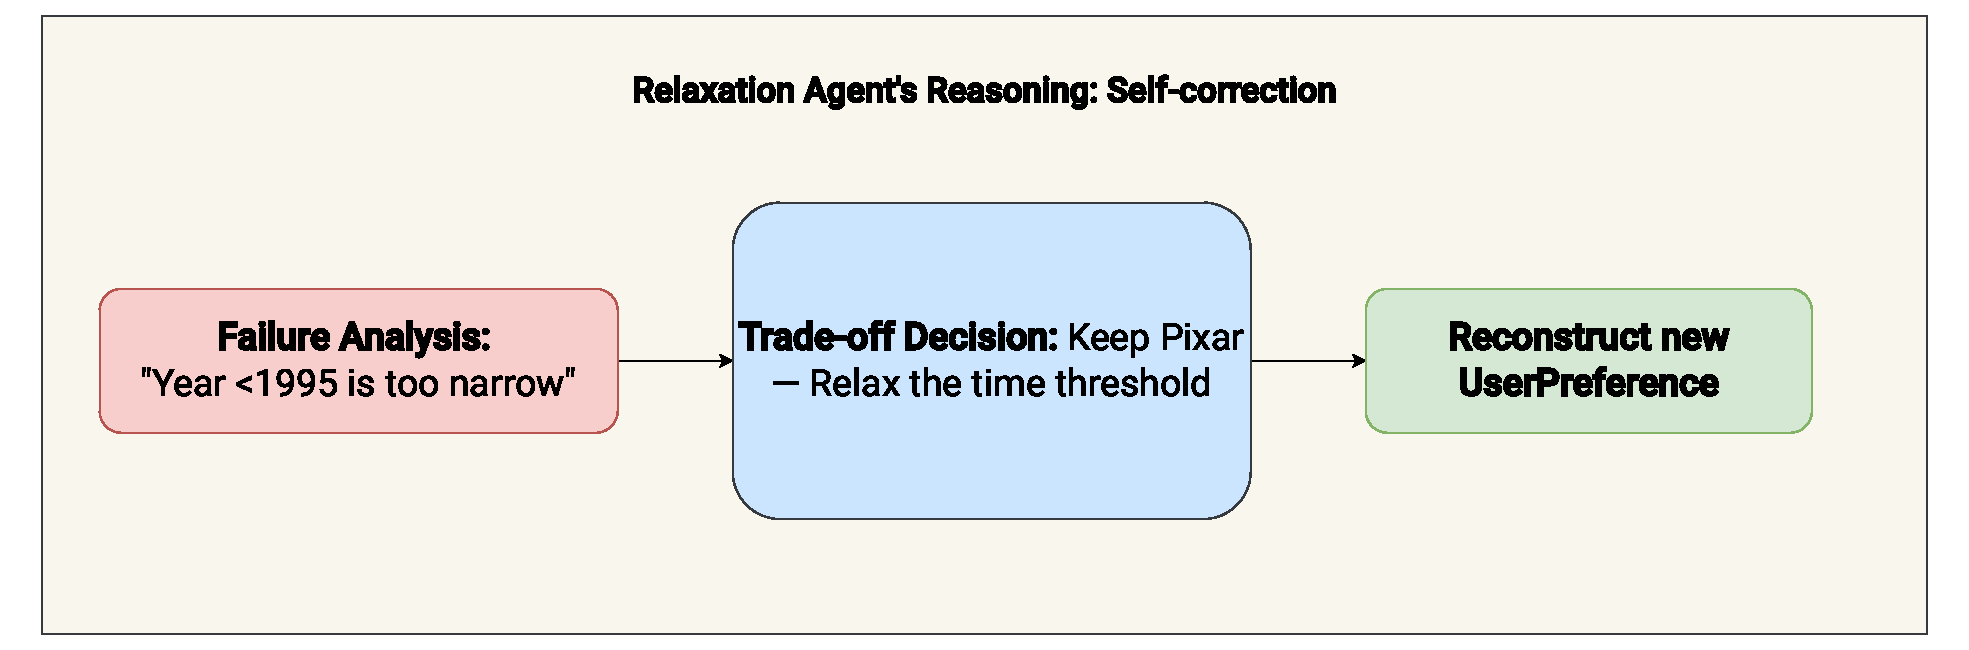
\includegraphics[width=\linewidth]{Chap4/images/relaxation_agent.pdf}
    \caption{Quy trình phân tích điểm nghẽn và tái cấu trúc ý định của Relaxation Agent. Dựa trên phân cấp ưu tiên (Sacrifice Hierarchy), tác tử nới lỏng các điều kiện tìm kiếm và khởi động lại vòng lặp hội thoại mới.}
    \label{fig:relaxation_agent}
\end{figure}

\subsection{Phân tích điểm nghẽn và Phân cấp ưu tiên (Sacrifice Hierarchy)}
Tác tử Thỏa hiệp tiếp nhận Báo cáo lỗi (Error Report) từ Critic Agent và tiến hành Phân tích điểm nghẽn (Bottleneck Analysis). Để hệ thống không rơi vào vòng lặp vô hạn (infinite loop) khi liên tục thử lại cùng một chiến lược thất bại, tác tử được trang bị một bộ nhớ trạng thái ngắn hạn (short-term state memory) để ghi nhận các ràng buộc đã từng được nới lỏng.

Cơ chế cốt lõi của bước này là việc xây dựng một cây \textbf{Phân cấp ưu tiên (Sacrifice Hierarchy)}. Tác tử sử dụng LLM để xác định các đặc trưng nào là "bất khả xâm phạm" (core properties) và đặc trưng nào mang tính thứ cấp (soft properties) dựa trên ngữ cảnh hội thoại. Ví dụ:
\begin{itemize}
    \item \textbf{Cốt lõi (Core):} Thể loại (Genre) thường là yếu tố quyết định. Nếu người dùng muốn xem "Phim Hài", hệ thống không được gợi ý "Phim Kinh dị".
    \item \textbf{Thứ cấp (Soft):} Niên đại phát hành (Release Year) hoặc điểm đánh giá (Rating) có thể được nới lỏng linh hoạt. Biên độ năm có thể được mở rộng từ $[2010, 2020]$ thành $[2005, 2025]$, hoặc hạ ngưỡng \texttt{min\_rating} từ $8.0$ xuống $7.5$.
\end{itemize}
Phương pháp thỏa hiệp tuần tự này dựa trên cơ sở tối ưu hóa hàm thỏa dụng dự kiến (expected utility) của người dùng, đảm bảo rằng kết quả trả về, dù không hoàn hảo 100\%, vẫn bám sát nhất có thể vào ý định gốc.

\subsection{Tái cấu trúc ý định (Intent Reconstruction)}
Sau khi thiết lập phương án thỏa hiệp dựa trên Sacrifice Hierarchy, Relaxation Agent tiến hành \textbf{Tái cấu trúc ý định (Intent Reconstruction)}. Quá trình này bao gồm hai thao tác:
\begin{enumerate}
    \item Khởi tạo lại cấu trúc hồ sơ sở thích (UserPreference JSON) với các ràng buộc đã được nới lỏng.
    \item Cập nhật lại danh sách truy vấn ngữ nghĩa (Multi-Queries) để phù hợp với hướng tiếp cận mới.
\end{enumerate}
Bản thiết kế mới này được đẩy ngược trở lại Orchestrator Agent, tự động kích hoạt vòng lặp tìm kiếm lần thứ hai (Attempt 2). Điểm đặc biệt của kiến trúc đa tác tử ARGOS là khả năng \textbf{tự phục hồi (self-healing)}. Khi kết quả cuối cùng được trả về cho người dùng, hệ thống luôn đính kèm một \textit{diễn giải logic phân nhánh (branching explanation)}, ví dụ: \textit{"Tôi không tìm thấy phim hoạt hình Pixar nào trước năm 1995, nhưng đây là một số tác phẩm xuất sắc của Studio Ghibli trong cùng thời kỳ"}. Cách diễn đạt này thừa nhận minh bạch giới hạn dữ liệu đồng thời vẫn mang lại gợi ý có giá trị, duy trì sự thông suốt của mạch hội thoại (Conversation Flow).

\section{Cải tiến Module Xếp hạng hai giai đoạn (Decoupled Reranking)}
GRACE sử dụng một Generative LLM duy nhất để xếp hạng toàn bộ danh sách ứng viên, hiệu quả nhưng chi phí tính toán tăng nhanh khi số ứng viên lớn. ARGOS cải tiến bằng cách phân tách thành hai giai đoạn, mỗi giai đoạn dùng mô hình phù hợp với yêu cầu tốc độ và độ sâu suy luận riêng biệt.

Sự cần thiết của phương pháp này xuất phát từ hai hạn chế cốt lõi của Generative LLM:
\begin{enumerate}
    \item \textbf{Hiện tượng Lost-in-the-Middle:} Khi đưa một danh sách dài hàng trăm ứng viên vào ngữ cảnh (context window) của LLM, mô hình thường chỉ tập trung vào các kết quả ở đầu và cuối văn bản, bỏ qua các thông tin quan trọng ở giữa.
    \item \textbf{Độ phức tạp tính toán (Computational Complexity):} Việc áp dụng cơ chế Self-Attention trên toàn bộ chuỗi văn bản của hàng trăm siêu dữ liệu phim sẽ dẫn đến phức tạp tính toán bậc hai ($O(N^2)$), tăng đáng kể chi phí API và độ trễ.
\end{enumerate}

Để giải quyết, quy trình Decoupled Reranking được thiết kế như sau:
\begin{itemize}
    \item \textbf{Giai đoạn 1 - Lọc nhanh với Cross-Encoder (SLM Reranker):} Ở giai đoạn này, hệ thống ứng dụng một mô hình ngôn ngữ quy mô nhỏ (Small Language Model - SLM) chuyên dụng cho tác vụ xếp hạng. Khác với Bi-Encoder (tìm kiếm vector) tính toán độc lập điểm số của truy vấn và tài liệu, Cross-Encoder nối trực tiếp truy vấn $q$ và tài liệu $d$ để đánh giá mức độ tương đồng ngữ nghĩa sâu: $\text{Score} = \text{SLM}(q \oplus d)$. Mô hình này đánh giá cực kỳ nhanh danh sách hàng trăm ứng viên thu được từ pha Orchestrator và chỉ giữ lại tập hợp $\text{Top-}20$ sắc bén nhất.
    \item \textbf{Giai đoạn 2 - Suy luận Logic với Generative LLM:} Danh sách $\text{Top-}20$ đã được tinh gọn sẽ được chuyển giao cho LLM cấu trúc lớn (Large Language Model) để thực hiện suy luận logic cuối cùng. Tại đây, LLM không chỉ đối sánh ngữ nghĩa mà còn cân nhắc tính đa dạng (Diversity), sự bất ngờ (Serendipity) và lịch sử hội thoại để chọn lọc ra $\text{Top-}5$ kết quả xuất sắc nhất trình bày cho người dùng.
\end{itemize}
Cải tiến này khai thác tối đa lợi thế tốc độ của mô hình truy xuất chuyên dụng (SLM) đồng thời bảo toàn năng lực biện luận bậc cao của mô hình sinh ngôn ngữ (LLM). Việc thiết lập $K_1 = 20$ và $K_2 = 5$ là điểm cân bằng giữa tỷ lệ bao phủ (Recall) và thời gian phản hồi, được xác nhận qua phân tích thực nghiệm tại Chương 5. Quy trình xếp hạng hai giai đoạn này được tổng quát hóa trong Hình \ref{fig:argos_reranker}.


\begin{figure}[H]
    \centering
    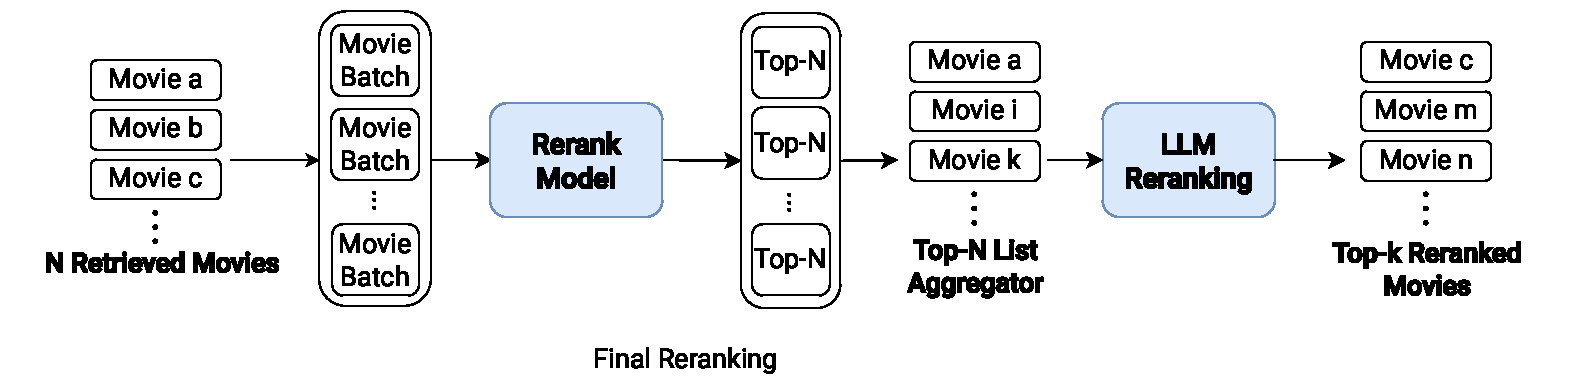
\includegraphics[width=\linewidth]{Chap4/images/Reranker.pdf}
    \caption{Quy trình xếp hạng hai giai đoạn (2-stage Reranking). Hệ thống kết hợp mô hình Rerank chuyên dụng để lọc nhanh danh sách ứng viên, sau đó tận dụng LLM để đánh giá sâu logic và đưa ra kết quả cuối cùng.}
    \label{fig:argos_reranker}
\end{figure}

\subsection{Sinh phản hồi hội thoại (Dialogue Response Generation)}
Sau khi Decoupled Reranking hoàn tất, danh sách $\text{Top-}5$ ứng viên cùng lịch sử hội thoại $C_t$ được chuyển giao cho Generative LLM để sinh phản hồi ngôn ngữ tự nhiên. Thay vì chỉ liệt kê tên phim, LLM tổng hợp lý do gợi ý từ các đặc trưng đã trích xuất (thể loại, đạo diễn, bầu không khí), tạo ra phản hồi cá nhân hóa và có thể giải thích được (Explainable Recommendation). Nếu Relaxation Agent đã nới lỏng một ràng buộc trong lượt truy xuất, thông tin về thỏa hiệp đó được đưa vào prompt để LLM sinh diễn giải phù hợp, ví dụ: \textit{"Không tìm thấy phim của Nolan phát hành sau 2020, nhưng đây là ba tác phẩm mang phong cách tương tự gần nhất."}\ Cơ chế này khép kín toàn bộ luồng xử lý của ARGOS từ ý định người dùng đến phản hồi hội thoại cuối cùng.

\section*{Kết luận chương}

Chương 4 đã trình bày chi tiết về thiết kế cấu trúc và luồng vận hành của hệ thống đa tác tử ARGOS. Bằng cách thay thế mô hình đường ống tĩnh một chiều, ARGOS xây dựng một quy trình cộng tác phân tán: bắt đầu từ khâu phân rã ý định và dự báo trọng số của \textit{Profiler Agent}, quá trình suy luận cấu trúc của \textit{Graph Agent}, khả năng điều phối của \textit{Orchestrator Agent}, cho đến các cơ chế kiểm soát chất lượng chặt chẽ của \textit{Critic Agent} và \textit{Relaxation Agent}. Cấu trúc này, khi kết hợp cùng phương pháp Xếp hạng hai giai đoạn (Decoupled Reranking), nhằm mục tiêu tối ưu hóa sự cân bằng giữa tính chính xác và độ trễ tính toán. Hiệu năng thực tiễn của kiến trúc này sẽ được định lượng và phân tích chi tiết thông qua các bài toán đánh giá thực nghiệm trong Chương 5.